\SourcePage{264}
\SGAchapter{XVIII}{Lefschetz 铅笔的上同调研究}{Étude cohomologique des pinceaux de Lefschetz}
\begin{center}N. Katz\footnote{根据 Grothendieck 的简要笔记。}\end{center}
% 原书本讲目录在此页；由译本的章节目录重建。
\SourcePage{265}
\textbf{引言}

本讲给出 \Term{lefschetz-pencil}{Lefschetz 铅笔}的初等\Term{cohomology}{上同调}结构。第1—4节叙述关于\Term{projective-bundle}{射影丛}和\Term{blow-up}{爆破}的\Term{cohomology}{上同调}结构的那些“众所周知”的事实。第5节进行标题所指的研究，其假设是 $X$ 满足“\Term{lefschetz-cow-theorem}{Lefschetz 牛定理}”（5.2），并且所考察的\Term{pencil}{铅笔} $D$ 满足一个在 $D$ 上具有\Term{local-nature}{局部性质}的条件 (A)（5.3）。主要结果是 5.6、5.7 和 5.8.7；最后一个结果在第 XX 讲的 Griffiths \Term{theorem}{定理}的证明中起着关键\Term{action}{作用}。最后一节的内容显然较不初等；我们利用 Raynaud 夫人在 SGA 1 第 XIII 讲关于“\Term{tame-fundamental-group}{温和基本群}”的论述，以及 \Term{picard-lefschetz-formula}{Picard--Lefschetz 公式}（第 XVI 讲），证明：
\begin{enumerate}
\item 条件 (A) 往往成立（6.3、6.4）；
\item 除了 $\dim(X)$ 为奇数且\Term{characteristic}{特征}为 $2$ 的情形，\Term{lefschetz-pencil}{Lefschetz 铅笔}的\Term{monodromy-group}{单值群}在“\Term{vanishing-cohomology}{消失上同调}”上的\Term{action}{作用}是\Term{irreducible}{不可约}的，并且它在经由 \Term{picard-lefschetz-formula}{Picard--Lefschetz 公式}与\Term{pencil}{铅笔}的各个“\Term{critical-point}{临界点}”相联系的“\Term{local-vanishing-cycle}{局部消失圈}”\Term{set}{集合}上的\Term{action}{作用}，在不计\Term{signature}{符号}的意义下是\Term{transitive-action}{传递}的（6.6 和 6.7）。
\end{enumerate}
\SourcePage{266}
\SGAsection{1}{射影丛的上同调}
\begin{SGAresult}{\Term{theorem}{定理}}{1.1（Deligne）}
设 $f:X\to S$ 是\Term{proper}{固有}\Term{morphism}{态射}，$\ell$ 是在 $S$ 上\Term{invertible}{可逆}的素数，$u\in H^2(X,\mathbf Z_\ell(1))$（相应地 $u\in H^2(X,\mathbf Q_\ell(1))$）是 $X$ 上的一个\Term{cohomology-class}{上同调类}，$\mathscr F$ 是 $X$ 上的一个 $\mathbf Z_\ell$-\Term{sheaf}{层}（相应地 $\mathbf Q_\ell$-\Term{sheaf}{层}）。假设存在整数 $n$，使得对每个整数 $j$ 和每个整数 $i>0$，映射
\[
 R^{n-i}f_*(\mathscr F(j))\xrightarrow{\ \wedge u^i\ }R^{n+i}f_*(\mathscr F(j+i))\tag{1.1.1}
\]
都是 $S$ 上的 $\mathbf Z_\ell$-\Term{sheaf}{层}（相应地 $\mathbf Q_\ell$-\Term{sheaf}{层}）的\Term{isomorphism}{同构}。那么，对于每个\Term{morphism}{态射} $g:S\to T$，\Term{leray-spectral-sequence}{Leray 谱序列}
\[
 E_2^{p,q}=R^pg_*R^qf_*(\mathscr F)\Longrightarrow R^{p+q}(gf)_*(\mathscr F)
\]
\Term{degenerate-spectral-sequence}{退化}。
\end{SGAresult}
证明见 [1，命题 2.4]。注意，根据\Term{proper-base-change}{固有基变换定理}（SGA 4 第 XII 讲 5.2），上述假设可以逐\Term{fibre}{纤维}检验。

\SourcePage{267}
\begin{SGAresult}{\Term{theorem}{定理}}{1.2（参见 SGA 5 第 VII 讲 2.2.1）}
设 $\mathscr E\to X$ 是一个\Term{vector-bundle}{向量丛}，\Term{locally-free}{局部自由}且\Term{rank}{秩}为 $1+r$。记 $f:\mathbf P(\mathscr E)\to X$ 为 $\mathscr E$ 所定义的\Term{projective-bundle}{射影丛}，$u\in H^2(\mathbf P(\mathscr E),\mathbf Z_\ell(1))$ 为\Term{canonical}{典范}\Term{invertible-sheaf}{可逆层} $\mathscr O_{\mathbf P(\mathscr E)}(1)$ 的\Term{first-chern-class}{第一 Chern 类}。那么，对于在 $X$ 上\Term{invertible}{可逆}的素数 $\ell$，有：

\textup{a)} \Term{spectral-sequence}{谱序列}
\[
 E_2^{p,q}=H^p(X,R^qf_*\mathbf Z_\ell)\Longrightarrow H^{p+q}(\mathbf P(\mathscr E),\mathbf Z_\ell)\tag{1.2.1}
\]
\Term{degenerate-spectral-sequence}{退化}。

\textup{b)} 由
\[
 \bigoplus T_{q-2j}\longmapsto \sum f^*(T_{q-2j})\wedge u^j
\]
定义的\Term{arrow}{箭头}
\[
 \bigoplus_{0\leq j\leq n}H^{q-2j}(X,\mathbf Z_\ell(-j))\longrightarrow H^q(\mathbf P(\mathscr E),\mathbf Z_\ell)\tag{1.2.2}
\]
是\Term{isomorphism}{同构}。
\end{SGAresult}
\begin{proof}
$f$ 的\Term{fibre}{纤维}是\Term{dimension}{维数}为 $r$ 的\Term{projective-space}{射影空间}，所以有
\[
 R^if_*\mathbf Z_\ell\xleftarrow[\sim]{\ \wedge u^{i/2}\ }
 \begin{cases}\mathbf Z_\ell(-i/2),&i\text{ 为偶数， }0\leq i\leq 2r,\\0,&\text{其他情形。}\end{cases}\tag{1.2.3}
\]
\Term{theorem}{定理} 1.1 适用于 $(f,\ell,u,\mathbf Z_\ell,r)$，从而得到 a)。根据 (1.2.3)，有
\SourcePage{268}
\[
 E_2^{a,b}=\begin{cases}H^a(X,\mathbf Z_\ell(-b/2)),&b\text{ 为偶数， }0\leq b\leq 2r,\\0,&\text{其他情形，}\end{cases}\tag{1.2.4}
\]
因此，$H^q(\mathbf P(\mathscr E),\mathbf Z_\ell)$ 关于此\Term{spectral-sequence}{谱序列}所给\Term{filtration}{滤过}的\Term{associated-graded}{伴随分次}是 $\bigoplus_{0\leq j\leq r}H^{q-2j}(X,\mathbf Z_\ell(-j))$。在这个\Term{direct-sum}{直和}上赋予\Term{filtration}{滤过}
\[
 F^i=\bigoplus_{\substack{0\leq j\leq r\\q-2j\geq i}}H^{q-2j}(X,\mathbf Z_\ell(-j)),
\]
立刻看出，\Term{arrow}{箭头} (1.2.2) 与\Term{filtration}{滤过}相容，并且在\Term{associated-graded}{伴随分次}上诱导\Term{identity-map}{恒等映射}，从而得到 b)。
\end{proof}

\SGAsection{2}{爆破簇的上同调（参见 SGA 5 第 VII 讲 8）}
\textbf{2.1。} 设 $X$ 是域 $k$ 上的\Term{smooth}{光滑}\Term{scheme}{概形}，$\Delta\subset X$ 是一个处处\Term{codimension}{余维数}为 $1+r$ 的\Term{smooth}{光滑}\Term{scheme}{概形}。已知（EGA IV 19.4.9）存在一个\Term{smooth}{光滑}\Term{scheme}{概形} $\widetilde X$，配有\Term{projective}{射影}\Term{morphism}{态射}
\[
 f:\widetilde X\longrightarrow X,\tag{2.1.1}
\]
使得置
\[
 \widetilde\Delta=f^{-1}(\Delta)=\Delta\times_X\widetilde X,\tag{2.1.2}
\]
则 $f$ 诱导一个\Term{isomorphism}{同构}
\[
 f|_{\widetilde X-\widetilde\Delta}:\widetilde X-\widetilde\Delta\xrightarrow{\sim}X-\Delta,\tag{2.1.3}
\]
并且 $\widetilde\Delta$ 与 $\check{\mathbf P}(N_{\Delta/X})$ 之间存在一个 $\Delta$-\Term{isomorphism}{同构}；这里后者是 $\Delta$ 在 $X$ 中的\Term{normal-bundle}{法丛} $N_{\Delta/X}$ 内诸直线所成的\Term{projective-bundle}{射影丛}。
\SourcePage{269}
因此有\Term{commutative-diagram}{交换图}
\[
\begin{tikzcd}
\widetilde\Delta\arrow[rr,"\sim"]\arrow[dr,"f|_{\widetilde\Delta}"']&&\check{\mathbf P}(N_{\Delta/X})\arrow[dl,"\text{典范投影}"]\\
&\Delta&
\end{tikzcd}\tag{2.1.4}
\]
\textbf{2.1.5。} 在特殊情形 $X=\operatorname{Spec}(A)$、$\Delta=\operatorname{Spec}(A/I)$，其中 $I=(g_0,\ldots,g_r)$ 时，可以用 Hopf 方法得到 $\widetilde X$（参见 EGA IV 19.4.11）：定义从 $X-\Delta$ 到 $\mathbf P^r$ 的\Term{morphism}{态射}
\[
 x\in X-\Delta\longmapsto(g_0(x),\ldots,g_r(x))\in\mathbf P^r,
\]
把它的\Term{graph}{图像} $\Gamma$ 看作\Term{embedding}{嵌入} $X\times\mathbf P^r$ 中。然后定义 $\widetilde X$ 为 $\Gamma$ 在 $X\times\mathbf P^r$ 中的\Term{schematic-closure}{概形闭包}；\Term{morphism}{态射} $f:\widetilde X\to X$ 是复合
\[
 \widetilde X\lhook\joinrel\longrightarrow X\times\mathbf P^r\xrightarrow{\operatorname{pr}_1}X.
\]
\textbf{2.1.6。} 类似地（仍参见 EGA IV 19.4.11），若 $X$ 是\Term{projective}{射影}的，且 $\Delta$ 是 $X$ 与 $1+r$ 个\Term{hypersurface}{超曲面}的交，设其方程为 $G_i=0$，$i=0,\ldots,r$，则仍考虑\Term{morphism}{态射}
\[
 X-\Delta\longrightarrow\mathbf P^r,\qquad x\in X-\Delta\longmapsto(G_0(x),\ldots,G_r(x)),
\]
并取其\Term{graph}{图像}在 $X\times\mathbf P^r$ 中的\Term{closure}{闭包}，得到 $\widetilde X$。具体地说，用 $\mathbf P^r$ 的\Term{homogeneous-coordinates}{齐次坐标} $\lambda_0,\ldots,\lambda_r$，$\widetilde X$ 是 $X\times\mathbf P^r$ 中由方程
\SourcePage{270}
\[
 \lambda_iG_j(x)=\lambda_jG_i(x),\qquad 0\leq i<j\leq r\tag{2.1.6.1}
\]
定义的\Term{scheme}{概形}。由这些方程可见，点 $(x,\lambda)$ 属于 $\widetilde\Delta$ 当且仅当 $x\in\Delta$；换言之，$\check{\mathbf P}(N_{\Delta/X})$ 是\Term{trivial-projective-bundle}{平凡射影丛}
\[
\begin{tikzcd}
\check{\mathbf P}(N_{\Delta/X})\arrow[rr,"\sim"]\arrow[dr,"\text{典范投影}"']&&\Delta\times\mathbf P^r\arrow[dl,"\operatorname{pr}_1"]\\
&\Delta&
\end{tikzcd}\tag{2.1.6.2}
\]
有如下\Term{commutative-diagram}{交换图}
\[
\begin{tikzcd}[column sep=large]
\Delta\times\mathbf P^r\arrow[r,"\sim"]\arrow[dr,"\operatorname{pr}_1"']&\widetilde\Delta\arrow[r,hook]\arrow[d,"f|_{\widetilde\Delta}"]&\widetilde X\arrow[r,hook]\arrow[d,"f"]&X\times\mathbf P^r\arrow[dl,"\operatorname{pr}_1"]\\
&\Delta\arrow[r,hook]&X&
\end{tikzcd}\tag{2.1.6.3}
\]
而复合\Term{inclusion}{包含映射} $\Delta\times\mathbf P^r\hookrightarrow X\times\mathbf P^r$ 是由 $\Delta\hookrightarrow X$ 经\Term{base-change}{基变换}得到的。

\begin{SGAresult}{\Term{theorem}{定理}}{2.2}
设 $X$ 是域 $k$ 上的\Term{smooth}{光滑}\Term{scheme}{概形}，$\Delta$ 是一个处处\Term{codimension}{余维数}为 $1+r$ 的\Term{smooth}{光滑}\Term{subscheme}{子概形}，$f:\widetilde X\to X$ 是 $X$ 沿 $\Delta$ 的\Term{blow-up}{爆破}。则：

\textup{(2.2.1)} \Term{leray-spectral-sequence}{Leray 谱序列}
\[
 E_2^{p,q}=H^p(X,R^qf_*\mathbf Z_\ell)\Longrightarrow H^{p+q}(\widetilde X,\mathbf Z_\ell)
\]
\Term{degenerate-spectral-sequence}{退化}。
\SourcePage{271}
\textup{(2.2.2)} 存在加法\Term{isomorphism}{同构}
\[
\begin{aligned}
H^q(\widetilde X,\mathbf Z_\ell)&\simeq H^q(X,\mathbf Z_\ell)\oplus\bigl(H^q(\widetilde\Delta,\mathbf Z_\ell)/\operatorname{Im}H^q(\Delta,\mathbf Z_\ell)\bigr)\\
&\simeq\bigoplus_{j=1}^r H^{q-2j}(\Delta,\mathbf Z_\ell(-j))\oplus H^q(X,\mathbf Z_\ell).
\end{aligned}
\]
\end{SGAresult}
\begin{proof}
记
\[
 g:\widetilde\Delta\longrightarrow\Delta\tag{2.2.3}
\]
为 $f$ 在 $\widetilde\Delta$ 上的\Term{restriction}{限制}，并以
\[
 j:\Delta\hookrightarrow X,\qquad i:\widetilde\Delta\hookrightarrow\widetilde X\tag{2.2.4}
\]
表示\Term{inclusion}{包含映射}，于是得到\Term{commutative-diagram}{交换图}
\[
\begin{tikzcd}
\widetilde X\arrow[d,"f"']&\widetilde\Delta\arrow[l,"i"']\arrow[d,"g"]\\
X&\Delta\arrow[l,"j"]
\end{tikzcd}\tag{2.2.5}
\]
它诱\Term{derive}{导出}\Term{morphism}{态射} $f$ 和 $g$ 以及 $\widetilde X$ 和 $\widetilde\Delta$ 上的\Term{sheaf}{层} $\mathbf Z_\ell$ 所对应的 \Term{leray-spectral-sequence}{Leray 谱序列}之间的\Term{homomorphism}{同态}
\[
 E_r^{p,q}(f)\xrightarrow{(i^*,j^*)}E_r^{p,q}(g).\tag{2.2.6}
\]
另一方面，$f$ 诱导 $\widetilde X-\widetilde\Delta$ 与 $X-\Delta$ 的\Term{isomorphism}{同构}，所以由\Term{proper-base-change}{固有基变换定理}可得
\SourcePage{272}
\[
 R^qf_*\mathbf Z_\ell\simeq
 \begin{cases}\mathbf Z_\ell,&q=0,\\j_*R^qg_*\mathbf Z_\ell,&q>0,\end{cases}\tag{2.2.7}
\]
从而
\[
 E_2^{p,q}(f)\xrightarrow[\sim]{(i^*,j^*)}E_2^{p,q}(g),\qquad q\ne0.\tag{2.2.8}
\]
我们对 $r$ 归纳，证明
\[
 E_r^{p,q}(f)\xrightarrow[\sim]{(i^*,j^*)}E_r^{p,q}(g),\qquad q\ne0,\ r\geq2,\tag{2.2.9}
\]
以及
\[
 d_r^{p,q}(f)=0,\qquad r\geq2.\tag{2.2.10}
\]
暂且承认公式
\[
 d_r^{p,r-1}(f)=0,\qquad r\geq2,\ \text{任意 }p.\tag{2.2.11}
\]
先看 $r=2$。有\Term{commutative-diagram}{交换图}
\[
\begin{tikzcd}
E_2^{p,q}(f)\arrow[r,"{(i^*,j^*)}"]\arrow[d,"{d_2^{p,q}(f)}"']&E_2^{p,q}(g)\arrow[d,"{0=d_2^{p,q}(g)}"]\\
E_2^{p+2,q-1}(f)\arrow[r,"{(i^*,j^*)}"]&E_2^{p+2,q-1}(g)
\end{tikzcd}\tag{2.2.12}
\]
当 $q\leq0$ 时，$E_2^{p+2,q-1}(f)=0$，故 $d_2^{p,q}(f)=0$。当 $q=1$ 时，由 (2.2.11) 有 $d_2^{p,1}(f)=0$；当 $q>1$ 时，(2.2.12) 中的水平\Term{arrow}{箭头}都是\Term{isomorphism}{同构}，并由 1.2 和 2.1.4 知道 $d_2^{p,q}(g)=0$。这证明了 $r=2$ 时的 (2.2.10)，而 $r=2$ 时的 (2.2.9) 就是 (2.2.8)。
\SourcePage{273}
现设对于某个 $r\geq2$ 已知 (2.2.9) 和 (2.2.10)。(2.2.10) 意味着 $E_r^{p,q}(f)\simeq E_{r+1}^{p,q}(f)$，而由 1.2 有 $E_r^{p,q}(g)\simeq E_{r+1}^{p,q}(g)$，因而得到\Term{commutative-diagram}{交换图}
\[
\begin{tikzcd}
E_r^{p,q}(f)\arrow[r,"{(i^*,j^*)}"]\arrow[d,"\sim"']&E_r^{p,q}(g)\arrow[d,"\sim"]\\
E_{r+1}^{p,q}(f)\arrow[r,"{(i^*,j^*)}"]&E_{r+1}^{p,q}(g).
\end{tikzcd}\tag{2.2.13}
\]
结合 $r$ 时的 (2.2.9)，这就给出 $r+1$ 时的 (2.2.9)。为\Term{pushout}{推出} $r+1$ 时的 (2.2.10)，考察\Term{commutative-diagram}{交换图}
\[
\begin{tikzcd}
E_{r+1}^{p,q}(f)\arrow[r,"{(i^*,j^*)}"]\arrow[d,"{d_{r+1}^{p,q}(f)}"']&E_{r+1}^{p,q}(g)\arrow[d,"{0=d_{r+1}^{p,q}(g)}"]\\
E_{r+1}^{p+r+1,q-r}(f)\arrow[r,"{(i^*,j^*)}"]&E_{r+1}^{p+r+1,q-r}(g).
\end{tikzcd}\tag{2.2.14}
\]
当 $q\leq r-1$ 时，$E_{r+1}^{p+r+1,q-r}(f)=0$，所以 $d_r^{p,q}(f)=0$。当 $q=r$ 时，由 (2.2.11) 得到结论；当 $q>r$ 时，(2.2.14) 中的水平\Term{arrow}{箭头}都是\Term{isomorphism}{同构}，且由 1.2 有 $d_{r+1}^{p,q}(g)=0$，故得所需结论。

剩下的是证明 (2.2.11)，它就是说复合的“\Term{edge-homomorphism}{边缘同态}”
\[
 E_2^{p,0}(f)\longrightarrow E_3^{p,0}(f)\longrightarrow E_4^{p,0}(f)\longrightarrow\cdots\longrightarrow E_\infty^{p,0}(f)\tag{2.2.15}
\]
是\Term{isomorphism}{同构}，也就是说
\[
 f^*:H^p(X,\mathbf Z_\ell)\longrightarrow H^p(\widetilde X,\mathbf Z_\ell)\tag{2.2.16}
\]
是\Term{injective}{单射}。
\SourcePage{274}
但它存在\Term{left-inverse}{左逆}，即 \Term{gysin-homomorphism}{Gysin 同态}（SGA 5 第 IV 讲）
\[
 f_*:H^p(\widetilde X,\mathbf Z_\ell)\longrightarrow H^p(X,\mathbf Z_\ell),\tag{2.2.17}
\]
而且确有
\[
 f_*f^*=\operatorname{id}.\tag{2.2.18}
\]
这由\Term{projection-formula}{投影公式}以及 $f_*(1)=1$ 得到；后一事实是因为 $f$ 是\Term{birational}{双有理}的，因而\Term{degree}{次数}为一。

这证明了 (2.2.1)。至于 (2.2.2)，注意图 (2.2.5) 在取\Term{cohomology}{上同调}后给出\Term{commutative-diagram}{交换图}
\[
\begin{tikzcd}
H^p(\widetilde X,\mathbf Z_\ell)\arrow[r,"i^*"]&H^p(\widetilde\Delta,\mathbf Z_\ell)\\
H^p(X,\mathbf Z_\ell)\arrow[u,"f^*"]\arrow[r,"j^*"']&H^p(\Delta,\mathbf Z_\ell)\arrow[u,"g^*"'].
\end{tikzcd}\tag{2.2.19}
\]
因此得到\Term{morphism}{态射}
\[
 \frac{H^p(\widetilde X,\mathbf Z_\ell)}{f^*H^p(X,\mathbf Z_\ell)}\xrightarrow{(i^*,j^*)}\frac{H^p(\widetilde\Delta,\mathbf Z_\ell)}{g^*H^p(\Delta,\mathbf Z_\ell)}.\tag{2.2.20}
\]
以 $F^i$ 表示由 \Term{leray-spectral-sequence}{Leray 谱序列}给出的 $H^\bullet(\widetilde X,\mathbf Z_\ell)$ 和 $H^\bullet(\widetilde\Delta,\mathbf Z_\ell)$ 的\Term{filtration}{滤过}，则 (2.2.20) 可重写为
\SourcePage{275}
\[
 \frac{H^p(\widetilde X,\mathbf Z_\ell)}{F^pH^p(\widetilde X,\mathbf Z_\ell)}\xrightarrow{(i^*,j^*)}\frac{H^p(\widetilde\Delta,\mathbf Z_\ell)}{F^pH^p(\widetilde\Delta,\mathbf Z_\ell)}.\tag{2.2.21}
\]
根据 (2.2.9)，\Term{arrow}{箭头} (2.2.21) 在\Term{associated-graded}{伴随分次}上是\Term{isomorphism}{同构}，因此 (2.2.20) 是\Term{isomorphism}{同构}。另一方面，(2.2.18) 给出\Term{direct-sum-decomposition}{直和分解}
\[
\begin{tikzcd}[column sep=huge]
H^\bullet(\widetilde X,\mathbf Z_\ell)\arrow[r,shift left=1.1ex,"{f_*\oplus(1-f^*f_*)}"]&H^\bullet(X,\mathbf Z_\ell)\oplus\operatorname{Ker}f_*\arrow[l,shift left=1.1ex,"{f^*+\text{包含映射}}"]
\end{tikzcd}\tag{2.2.22}
\]
而 (1.2.2) 给出\Term{direct-sum-decomposition}{直和分解}
\[
 \frac{H^\bullet(\widetilde\Delta,\mathbf Z_\ell)}{g^*H^\bullet(\Delta,\mathbf Z_\ell)}\xleftarrow{\sim}\bigoplus_{1\leq j\leq r}H^{\bullet-2j}(\Delta,\mathbf Z_\ell(-j)).\tag{2.2.23}
\]
把\Term{isomorphism}{同构} (2.2.20) 与\Term{resolution}{分解} (2.2.22)、(2.2.23) 合起来，就得到 (2.2.2)。证毕。
\end{proof}

\textbf{注记 2.2.24。} 略述 (2.2.2) 的第二种证明，它显然简单得多，适用于 $X$ 在 $k$ 上\Term{proper}{固有}的情形。更\Term{generic}{一般}地，不对 $X$ 作假设，可以在\Term{cohomology-with-proper-support}{固有支撑上同调}中得到相应结果 (2.2.26)。对于 $(\widetilde X,\widetilde\Delta)$ 和 $(X,\Delta)$，有“\Term{cohomology-with-proper-support}{固有支撑上同调}”（记为 $H_c^\bullet$）的\Term{exact-sequence}{正合列}，它们组成\Term{commutative-diagram}{交换图}
\SourcePage{276}
\[
\begin{tikzcd}[column sep=small]
\cdots\arrow[r]&H_c^i(\widetilde X-\widetilde\Delta,\mathbf Z_\ell)\arrow[r]&H_c^i(\widetilde X,\mathbf Z_\ell)\arrow[r]&H_c^i(\widetilde\Delta,\mathbf Z_\ell)\arrow[r]&H_c^{i+1}(\widetilde X-\widetilde\Delta,\mathbf Z_\ell)\arrow[r]&\cdots\\
\cdots\arrow[r]&H_c^i(X-\Delta,\mathbf Z_\ell)\arrow[u,"\sim"]\arrow[r]&H_c^i(X,\mathbf Z_\ell)\arrow[u,"f^*"]\arrow[r]&H_c^i(\Delta,\mathbf Z_\ell)\arrow[u,"g^*"]\arrow[r]&H_c^{i+1}(X-\Delta,\mathbf Z_\ell)\arrow[u,"\sim"]\arrow[r]&\cdots
\end{tikzcd}\tag{2.2.25--2.2.26}
\]
把\Term{acyclic-complex}{无上同调复形} (2.2.25) 除以\Term{acyclic-complex}{无上同调子复形} (2.2.26)，得到\Term{acyclic-complex}{无上同调复形}
\[
 \cdots\longrightarrow0\longrightarrow\frac{H_c^i(\widetilde X,\mathbf Z_\ell)}{f^*H_c^i(X,\mathbf Z_\ell)}\longrightarrow\frac{H_c^i(\widetilde\Delta,\mathbf Z_\ell)}{g^*H_c^i(\Delta,\mathbf Z_\ell)}\longrightarrow0\longrightarrow\cdots.\tag{2.2.27}
\]
也就是说，无须考虑\Term{spectral-sequence}{谱序列}，便得到 (2.2.20) 是\Term{isomorphism}{同构}。此后，刚才的论证就适用，并给出 (2.2.2)。

\begin{SGAresult}{推论}{2.3}
置
\[
 b_q(X)=\dim_{\mathbf Q_\ell}H^q(X,\mathbf Q_\ell),\qquad \chi(X)=\sum(-1)^qb_q(X).
\]
则有
\[
 b_q(\widetilde X)=b_q(X)+\sum_{j=1}^r b_{q-j}(\Delta),\tag{2.3.1}
\]
\[
 \chi(\widetilde X)=\chi(X)+r\chi(\Delta).\tag{2.3.2}
\]
\end{SGAresult}

\SourcePage{277}
\SGAsection{3}{与铅笔相联系的爆破}
\textbf{3.1。} 设 $X$ 是\Term{algebraically-closed-field}{代数闭域} $k$ 上的\Term{projective}{射影}、\Term{smooth}{光滑}、\Term{irreducible}{不可约}\Term{algebraic-variety}{簇}，\Term{dimension}{维数}为 $n$，而 $D=[H_\tau]_{\tau\in\mathbf P^1}$ 是一个\Term{hypersurface}{超曲面}\Term{pencil}{铅笔}，其\Term{pencil-axis}{轴}与 $X$ \Term{transverse-intersection}{横截相交}于 $\Delta$。现在考虑 $X$ 沿 $\Delta$ 的\Term{blow-up}{爆破}，并给出其显式描述。

就方程而言，以 $(\lambda,\mu)$ 表示 $\mathbf P^1$ 的\Term{homogeneous-coordinates}{齐次坐标}，以 $F,G$ 表示使 $F=G=0$ 定义\Term{pencil}{铅笔}的\Term{pencil-axis}{轴}的两个\Term{linear-form}{线性形式}，则\Term{pencil}{铅笔}写作
\[
 \lambda F-\mu G.\tag{3.1.1}
\]
\Term{subscheme}{子概形} $\Delta$ 按定义是 $X$ 与\Term{linear-subvariety}{线性子簇} $G=F=0$ 的交。根据 2.1.6，
\[
 \widetilde X=\{(x,(\lambda,\mu))\in X\times\mathbf P^1\mid\lambda F-\mu G=0\};\tag{3.1.2}
\]
它是映射
\[
 X-\Delta\longrightarrow\mathbf P^1,\qquad x\longmapsto(G(x),F(x))\tag{3.1.3}
\]
的\Term{graph}{图像}在 $X\times\mathbf P^1$ 中的\Term{schematic-closure}{概形闭包}。

$\widetilde X$ 的主要优点在于，它是 $k$ 上的\Term{projective}{射影}\Term{smooth}{光滑}\Term{algebraic-variety}{簇}（\Term{projective}{射影}性来自它\Term{embedding}{嵌入}于 $X\times\mathbf P^1$，\Term{smooth}{光滑}性来自 $\Delta$ 的\Term{smooth}{光滑}性），并且存在到 $\mathbf P^1$ 的\Term{morphism}{态射} $\rho$，即
\[
 \rho:\widetilde X\hookrightarrow X\times\mathbf P^1\xrightarrow{\operatorname{pr}_2}\mathbf P^1,\tag{3.1.4}
\]
其\Term{fibre}{纤维}正是 $X$ 被我们的\Term{pencil}{铅笔}中各成员截出的\Term{hyperplane-section}{超平面截面}：
\[
 \rho^{-1}(t)=X_t\overset{\mathrm{def}}=X\cdot H_t.
\]

\SourcePage{278}
\textbf{3.2。\Term{dual-variety}{对偶簇}的\Term{degree}{次数}：\Term{topology}{拓扑}方法。}

进一步假设 3.1 中的\Term{pencil}{铅笔}满足：
\begin{description}
\item[(3.2.1)] 对 $\mathbf P^1$ 的某个\Term{nonempty}{非空}\Term{open-subset}{开子集}中的每个 $t$，$X_t$ 都是\Term{smooth}{光滑}的；
\item[(3.2.2)] 如果 $X_t$ 是\Term{singular}{奇异}的，那么它只有\Term{nondegenerate-quadratic-singularity}{非退化二次奇点}（第 XVII 讲 1.1）。
\end{description}
特别地，若 $\operatorname{char}k\ne2$ 或 $X$ 的\Term{dimension}{维数}为偶数，则 \Term{lefschetz-pencil}{Lefschetz 铅笔}（第 XVII 讲 2.21）满足这些条件。

设 $\eta$ 是 $\mathbf P^1$ 的\Term{generic-point}{泛点}，$\bar\eta$ 是其上的一个\Term{geometric-point}{几何点}，$n$ 是 $X$ 的\Term{dimension}{维数}，$\chi$ 是取值于\Term{sheaf}{层} $\mathbf Q_\ell$ 的 \Term{euler-poincare-characteristic}{Euler--Poincaré 特征数}。将第 XVI 讲 2.1 的 \Term{euler-poincare-formula}{Euler--Poincaré 公式}用于\Term{morphism}{态射} $\rho$，得到
\[
 \chi(\widetilde X)=\chi(\mathbf P^1)\chi(X_{\bar\eta})+(-1)^n\sum_{\text{各纤维的奇点}}1.\tag{3.2.3}
\]
结合 (2.2.2)，此式改写为
\[
 (-1)^n[\text{奇点总数}]=\chi(X)+\chi(\Delta)-2\chi(X_{\bar\eta}).\tag{3.2.4}
\]
注意，量 $\chi(X)+\chi(\Delta)-2\chi(X_{\bar\eta})$ 与\Term{pencil}{铅笔}的具体选择无关，它只依赖于 $X$ 在某个 $\mathbf P^r$ 中的\Term{embedding}{嵌入}，甚至只依赖于 $\mathscr O_X(1)$ 的 \Term{chern-class}{Chern 类}，参见第 XVII 讲 5.7.5 和 5.7.6。

\SourcePage{279}
\textbf{3.2.5。} 用一个具体例子说明。取 $X=\mathbf P^2$，$\{H_\tau\}$ 是 $\mathbf P^2$ 中由\Term{degree}{次数}为 $d$ 的\Term{curve}{曲线}组成的\Term{pencil}{铅笔}，满足 (3.1)、(3.2.1) 和 (3.2.2)。有
\[
\begin{aligned}
\chi(X)&=3&&\text{（由 1.2），}\\
\chi(X_{\bar\eta})&=-d(d-3)&&\text{（参见 SGA 5 第 VII 讲 7.3），}\\
\chi(\Delta)&=d^2,
\end{aligned}\tag{3.2.6}
\]
从而
\[
 \text{奇点总数为 }3(d-1)^2.\tag{3.2.7}
\]
取特殊情形 $d=3$，考虑\Term{elliptic-curve}{椭圆曲线}族（\Term{characteristic}{特征}不等于 $3$）
\[
 X^3+Y^3+Z^3+3\mu XYZ.\tag{3.2.8}
\]
四条\Term{singular-fibre}{奇异纤维}位于 $\mu$ 为三次\Term{root-of-unity}{单位根}以及 $\mu=\infty$ 之处，每条\Term{singular-fibre}{奇异纤维}都是如下三条直线的并：
\[
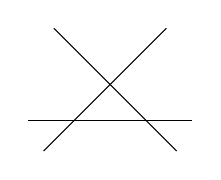
\begin{tikzpicture}[scale=.65]
\draw (-1.3,-.6)--(1.1,1.8);
\draw (-1.1,1.8)--(1.3,-.6);
\draw (-1.6,0)--(1.6,0);
\end{tikzpicture}\tag{3.2.9}
\]
它恰有三个\Term{singular-point}{奇点}，全是\Term{nondegenerate-quadratic-singularity}{非退化二次奇点}。合起来一共十二个\Term{singular-point}{奇点}，于是这个例子验证了 (3.2.7)。

\SourcePage{280}
\begin{SGAresult}{命题}{3.2.10}
设 $X\hookrightarrow\mathbf P^r$ 是一个 \Term{lefschetz-embedding}{Lefschetz 嵌入}（第 XVII 讲 2.3），并假设 $n=\dim X$ 为偶数，或者 $\operatorname{char}k\ne2$。那么，每个 \Term{lefschetz-pencil}{Lefschetz 铅笔}看成 $\check{\mathbf P}^r$ 中的直线时，都与 $\check X$ 交于
\[
 (-1)^n[\chi(X)+\chi(\Delta)-2\chi(X_{\bar\eta})]\tag{3.2.11}
\]
个点，并且与之\Term{transverse-intersection}{横截相交}（EGA IV 17.13.7）。
\end{SGAresult}
\begin{proof}
由假设，\Term{lefschetz-pencil}{Lefschetz 铅笔}的某条\Term{fibre}{纤维}的每个\Term{singular-point}{奇点}都是\Term{nondegenerate-quadratic-singularity}{非退化二次奇点}，所以可用 (3.2.4)，得知\Term{pencil}{铅笔} $D$ 中的\Term{singular-fibre}{奇异纤维}数（每条恰含一个\Term{singular-point}{奇点}）就是 (3.2.11) 的数。另一方面，\Term{fibre}{纤维} $X_\tau$ 是\Term{singular}{奇异}的当且仅当 $\tau\in\check X\cap D$。为看出相交的\Term{transversality}{横截性}，注意 (3.2.11) 的数与 \Term{lefschetz-pencil}{Lefschetz 铅笔}的具体选择无关；由于泛\Term{pencil}{铅笔}是 \Term{lefschetz-pencil}{Lefschetz 铅笔}，这个数就是 $\check X$ 的\Term{degree}{次数}（即它作为 $\check{\mathbf P}^r$ 中\Term{hypersurface}{超曲面}的\Term{degree}{次数}；若 $\dim\check X\leq r-2$，则依约定此数为 $0$）。但是，一条直线 $D$ 若与\Term{degree}{次数}为 $d>0$ 的\Term{hypersurface}{超曲面}交于 $d$ 个不同的点 $x_i$（$1\leq i\leq d$），那么相交必然是\Term{transverse-intersection}{横截}的。事实上，$D$ 与 $\check X$ 在任意 $x_i$ 处的\Term{intersection-multiplicity}{交重数} $\mu_i=\operatorname{rg}(D\cap\check X\mid x_i)$ 至少为 $1$，而 $\sum_{i=1}^d\mu_i=d$，因此对每个 $i$ 都有 $\mu_i=1$；也就是说，$D\cap\check X$ 是\Term{smooth}{光滑}的，很容易看出这\Term{equivalence}{等价}于\Term{transversality}{横截性}。
\end{proof}

\SourcePage{281}
\textbf{注记 3.2.12。} 对一个已经假设与 $\check X$ \Term{transverse-intersection}{横截相交}的 \Term{lefschetz-pencil}{Lefschetz 铅笔} $D$（只要 $D$ 足够\Term{generic}{一般}，这一条件总是成立），结果 3.2.10 也可看作第 XVII 讲 5.7.2 与第 XVII 讲 3.5 所含事实 $\deg\varphi=1$ 的合并。当然，这里通过第 XVI 讲 2.1 的 \Term{euler-poincare-formula}{Euler--Poincaré 公式}证明的事实——每个 \Term{lefschetz-pencil}{Lefschetz 铅笔} $D$ 都与 $\check X$ \Term{transverse-intersection}{横截相交}——也可以利用 $D$ 的\Term{pencil-axis}{轴}与 $X$ \Term{transverse-intersection}{横截相交}这一事实，直接用初等方法证明。

\SGAsection{4}{与铅笔相联系的爆破的上同调}
\textbf{4.1。} 重新考虑 3.1 的情形，将其概括为\Term{commutative-diagram}{交换图}（参见 2.1.6.3）：
\[
\begin{tikzcd}[column sep=large]
X\times\mathbf P^1&\widetilde X\arrow[l,"f\times\rho"']\arrow[d,"f"]\arrow[dl,"\rho"']&\widetilde\Delta\arrow[l,"i"']\arrow[d,"g"]\arrow[r,"{(g,\rho i)}"]&\Delta\times\mathbf P^1\\
\mathbf P^1&X&\Delta\arrow[l,"j"]&
\end{tikzcd}\tag{4.1.1}
\]
先把 (2.2.2) 在这种情形下写得更具体。

\begin{SGAresult}{命题}{4.2}
在 3.1 的假设下：

\textup{(4.2.1)} $\mathbf Z_\ell$-\Term{module}{模}的\Term{homomorphism}{同态}
\[
\begin{tikzcd}[column sep=huge]
H^\bullet(\widetilde X,\mathbf Z_\ell)\arrow[r,shift left=1.1ex,"{f_*\oplus(1-f^*f_*)}"]&H^\bullet(X,\mathbf Z_\ell)\oplus\operatorname{Ker}(f_*:H^\bullet(\widetilde X,\mathbf Z_\ell)\to H^\bullet(X,\mathbf Z_\ell))\arrow[l,shift left=1.1ex,"{f^*+\mathrm{incl}}"]
\end{tikzcd}
\]
\SourcePage{282}
是互逆的\Term{isomorphism}{同构}。

\textup{(4.2.2)} $\mathbf Z_\ell$-\Term{module}{模}的\Term{homomorphism}{同态}
\[
\begin{tikzcd}[column sep=huge]
H^\bullet(\widetilde X,\mathbf Z_\ell)\arrow[r,shift left=1.1ex,"{f_*\oplus(g_*i^*)}"]&H^\bullet(X,\mathbf Z_\ell)\oplus H^{\bullet-2}(\Delta,\mathbf Z_\ell(-1))\arrow[l,shift left=1.1ex,"{f^*+i_*g^*}"]
\end{tikzcd}
\]
是互逆的\Term{isomorphism}{同构}。

\textup{(4.2.3)} 通过 (4.2.2) 将 $H^\bullet(\widetilde X,\mathbf Z_\ell)$ 中的\Term{cup-product}{杯积}“搬运”到 $H^\bullet(X,\mathbf Z_\ell)\oplus H^{\bullet-2}(\Delta,\mathbf Z_\ell(-1))$ 上所得的\Term{algebra-structure}{代数结构}，用元素
\[
 a,b\in H^\bullet(X,\mathbf Z_\ell),\qquad x,y\in H^{\bullet-2}(\Delta,\mathbf Z_\ell(-1))
\]
表示为以下公式：
\[
 (0\oplus x)\wedge(0\oplus y)=-j_*(xy)\oplus2xy\,c_1(\mathscr O_\Delta(1)),\tag{4.2.3.1}
\]
\[
 (a\oplus0)\wedge(b\oplus0)=ab\oplus0,\tag{4.2.3.2}
\]
\[
 (a\oplus0)\wedge(0\oplus y)=0\oplus j^*(a)y,\tag{4.2.3.3}
\]
\[
 (0\oplus x)\wedge(b\oplus0)=0\oplus xj^*(b).\tag{4.2.3.4}
\]
特别地，对于
\[
\begin{aligned}
a\oplus x&\in H^\bullet(X,\mathbf Z_\ell)\oplus H^{\bullet-2}(\Delta,\mathbf Z_\ell(-1)),\\
b\oplus y&\in H^{2n-\bullet}(X,\mathbf Z_\ell)\oplus H^{2n-2-\bullet}(\Delta,\mathbf Z_\ell(-1)),
\end{aligned}
\]
\SourcePage{283}
有
\[
 (a\oplus x)\wedge(b\oplus y)=ab-j_*(xy).\tag{4.2.3.5}
\]
换言之，$H^\bullet(\widetilde X,\mathbf Z_\ell)$ 的总\Term{intersection-matrix}{交矩阵}写作
\[
 \begin{pmatrix}
 \text{$X$ 上的总交矩阵}&0\\
 0&-\text{$\Delta$ 上的总交矩阵}
 \end{pmatrix}.
\]
\end{SGAresult}
\begin{proof}
(4.2.1) 已经证明（参见 (2.2.22)）。对于 (4.2.2)，先注意到 $g:\widetilde\Delta\to\Delta$ 是\Term{rank}{秩}为一的\Term{projective-bundle}{射影丛}，因此列
\[
 0\longrightarrow H^\bullet(\Delta,\mathbf Z_\ell)\xrightarrow{g^*}H^\bullet(\widetilde\Delta,\mathbf Z_\ell)\xrightarrow{g_*}H^{\bullet-2}(\Delta,\mathbf Z_\ell(-1))\longrightarrow0\tag{4.2.4}
\]
是\Term{exact-sequence}{正合}的（参见 (1.2.2)）。结合 (2.2.26)，得到\Term{exact-sequence}{正合列}的\Term{commutative-diagram}{交换图}
\[
\begin{tikzcd}[column sep=small]
0\arrow[r]&H^\bullet(X,\mathbf Z_\ell)\arrow[r,"f^*"]\arrow[d,"j^*"']&H^\bullet(\widetilde X,\mathbf Z_\ell)\arrow[r,"g_*i^*"]\arrow[d,"i^*"']&H^{\bullet-2}(\Delta,\mathbf Z_\ell(-1))\arrow[r]\arrow[d,equal]&0\\
0\arrow[r]&H^\bullet(\Delta,\mathbf Z_\ell)\arrow[r,"g^*"]&H^\bullet(\widetilde\Delta,\mathbf Z_\ell)\arrow[r,"g_*"]&H^{\bullet-2}(\Delta,\mathbf Z_\ell(-1))\arrow[r]&0.
\end{tikzcd}\tag{4.2.5}
\]
\SourcePage{284}
利用\Term{splitting}{分裂} (4.2.1)，这就给出一个\Term{isomorphism}{同构}
\[
 f_*\oplus g_*i^*:H^\bullet(\widetilde X,\mathbf Z_\ell)\xrightarrow{\sim}H^\bullet(X,\mathbf Z_\ell)\oplus H^{\bullet-2}(\Delta,\mathbf Z_\ell(-1)).\tag{4.2.6}
\]
将 (4.2.5) \Term{transpose}{转置}，得到\Term{exact-sequence}{正合列}的\Term{commutative-diagram}{交换图}（作\Term{degree}{次数}变换 $\bullet\mapsto2n-\bullet$ 后）：
\[
\begin{tikzcd}[column sep=small]
0&H^\bullet(X,\mathbf Z_\ell)\arrow[l]&H^\bullet(\widetilde X,\mathbf Z_\ell)\arrow[l,"f_*"']&H^{\bullet-2}(\Delta,\mathbf Z_\ell(-1))\arrow[l,"i_*g^*"']&0\arrow[l]\\
0&H^{\bullet-2}(\Delta,\mathbf Z_\ell(-2))\arrow[l]\arrow[u,"j_*"]&H^{\bullet-2}(\widetilde\Delta,\mathbf Z_\ell(-1))\arrow[l,"g_*"']\arrow[u,"i_*"]&H^{\bullet-2}(\Delta,\mathbf Z_\ell(-1))\arrow[l,"g^*"']\arrow[u,equal]&0\arrow[l]
\end{tikzcd}\tag{4.2.7}
\]
于是得到一个\Term{isomorphism}{同构}
\[
 H^\bullet(X,\mathbf Z_\ell)\oplus H^{\bullet-2}(\Delta,\mathbf Z_\ell(-1))\xrightarrow{f^*+i_*g^*}H^\bullet(\widetilde X,\mathbf Z_\ell).\tag{4.2.8}
\]
剩下要证明复合
\[
\begin{aligned}
H^\bullet(X,\mathbf Z_\ell)\oplus H^{\bullet-2}(\Delta,\mathbf Z_\ell(-1))&\xrightarrow{f^*+i_*g^*}H^\bullet(\widetilde X,\mathbf Z_\ell)\\
&\xrightarrow{f_*\oplus(g_*i^*)}H^\bullet(X,\mathbf Z_\ell)\oplus H^{\bullet-2}(\Delta,\mathbf Z_\ell(-1))
\end{aligned}\tag{4.2.9}
\]
为\Term{identity-map}{恒等映射}。而有
\[
\begin{aligned}
f_*f^*&=\operatorname{id}\quad\text{在 }H^\bullet(X,\mathbf Z_\ell)\text{ 上，}& &\text{由 (2.2.18)，}\\
g_*i^*f^*&=0,&&\text{由 (4.2.5)，}\\
f_*i_*g^*&=0,&&\text{由 (4.2.7)，}
\end{aligned}
\]
所以只需证明
\[
 g_*i^*i_*g^*(x)=x,\qquad x\in H^\bullet(\Delta,\mathbf Z_\ell(-1)).\tag{4.2.10}
\]
\SourcePage{285}
为验证 (4.2.10)，先注意到 $i:\widetilde\Delta\hookrightarrow\widetilde X$ 是\Term{codimension}{余维数}为一的\Term{smooth}{光滑}\Term{subvariety}{子簇}的\Term{inclusion}{包含映射}，因此有 [SGA 5 第 VII 讲]
\[
 i^*i_*(x)=c_1(N_{\widetilde\Delta/\widetilde X})x,\tag{4.2.11}
\]
\[
 i_*(x)i_*(y)=i_*(xy\,c_1(N_{\widetilde\Delta/\widetilde X})).\tag{4.2.12}
\]
记 $\xi_X=\mathscr O_X(1)$、$\xi_\Delta=\mathscr O_\Delta(1)$、$\xi_{\mathbf P^1}=\mathscr O_{\mathbf P^1}(1)$ 等。由 EGA II 8.1.7，若 $\widetilde{\mathscr I}$ 是 $\widetilde\Delta$ 在 $\widetilde X$ 中的\Term{ideal}{理想}，则有
\[
\begin{aligned}
\check N_{\widetilde\Delta/\widetilde X}
&\simeq\widetilde{\mathscr I}/\widetilde{\mathscr I}^{\,2}
\simeq\widetilde{\mathscr I}\otimes_{\mathscr O_{\widetilde X}}\mathscr O_{\widetilde\Delta}\\
&\simeq\mathscr O_{\widetilde X}(1)\otimes_{\mathscr O_{\widetilde X}}\mathscr O_{\widetilde\Delta}
=\mathscr O_{\widetilde\Delta}(1),
\end{aligned}\tag{4.2.13}
\]
这里把 $\widetilde\Delta$ 解释为 $\mathbf P(\mathscr I/\mathscr I^2)$，其中 $\mathscr I$ 是 $\Delta$ 在 $X$ 中的\Term{ideal}{理想}。另一方面，有一个\Term{canonical}{典范}\Term{isomorphism}{同构}（因为 $\Delta$ 表示为 $X$ 与 $\mathbf P^r$ 中两个给定\Term{hyperplane}{超平面}的交）
\[
 \mathscr I/\mathscr I^2\simeq\mathscr O_\Delta^{\,2}(-1),
\]
它给出\Term{isomorphism}{同构}
\[
 \widetilde\Delta=\mathbf P(\mathscr I/\mathscr I^2)\simeq\mathbf P(\mathscr O_\Delta^{\,2}(-1))\xrightarrow[\sim]{\alpha}\mathbf P(\mathscr O_\Delta^{\,2})\simeq\Delta\times\mathbf P^1,
\]
其中 $\alpha$ 是 EGA II 4.1.4 中的\Term{canonical}{典范}\Term{isomorphism}{同构}。根据同处，此\Term{isomorphism}{同构}将
\[
 \mathscr O_{\widetilde\Delta}(1)=\mathscr O_{\mathbf P(\mathscr I/\mathscr I^2)}(1)=\mathscr O_{\mathbf P(\mathscr O_\Delta^{\,2}(-1))}(1)
\]
变为
\[
 \mathscr O_{\mathbf P(\mathscr O_\Delta^{\,2})}(1)\otimes_{\mathscr O_\Delta^{\,2}}\mathscr O_\Delta(-1)
 =\mathscr O_{\mathbf P^1}(1)\otimes_k\mathscr O_\Delta(-1),
\]
因此 (4.2.13) 写成
\[
 \check N_{\widetilde\Delta/\widetilde X}\simeq(\rho i)^*(\mathscr O_{\mathbf P^1}(1))\otimes g^*(\mathscr O_\Delta(-1)).\tag{4.2.14}
\]
对两边取 $c_1$，即得到以下\Term{lemma}{引理}。
\end{proof}

\SourcePage{286}
\begin{SGAresult}{\Term{lemma}{引理}}{4.3}
有
\[
 c_1(N_{\widetilde\Delta/\widetilde X})=g^*(\xi_\Delta)-(\rho i)^*(\xi_{\mathbf P^1}).
\]
\end{SGAresult}
\begin{proof}[续证命题 4.2]
回到 (4.2.10) 的证明。由 (4.2.11) 和 (4.3)，只需证明
\[
 g_*\bigl(g^*(x)[(\rho i)^*(c_1(\xi_{\mathbf P^1}))-g^*(c_1(\xi_\Delta))]\bigr)=x.
\]
由 (4.2.4)，$g_*g^*=0$，并且由于
\[
 \widetilde\Delta\xrightarrow[\sim]{g\times\rho i}\Delta\times\mathbf P^1,
\]
有
\[
 g_*\bigl(g^*(x)(\rho i)^*(c_1(\xi_{\mathbf P^1}))\bigr)=x,\tag{4.3.1}
\]
\[
 g_*\bigl(g^*(x)c_1(N_{\widetilde\Delta/\widetilde X})\bigr)=-x.\tag{4.3.2}
\]
现在计算通过 (4.2.2) 从\Term{cup-product}{杯积}搬运得到的 $H^\bullet(X,\mathbf Z_\ell)\oplus H^{\bullet-2}(\Delta,\mathbf Z_\ell(-1))$ 上的\Term{algebra-structure}{代数结构}。设 $a,b$ 是 $H^\bullet(X,\mathbf Z_\ell)$ 的元素，$x,y$ 是 $H^{\bullet-2}(\Delta,\mathbf Z_\ell(-1))$ 的元素。先证明 (4.2.3.1)。写作
\[
 (0\oplus x)\wedge(0\oplus y)=?\oplus?'.
\]
则
\[
\begin{aligned}
?&=f_*\bigl((i_*g^*(x))(i_*g^*(y))\bigr)\\
 &=f_*\bigl(i_*(g^*(xy)c_1(N_{\widetilde\Delta/\widetilde X}))\bigr)&&\text{由 (4.2.12)}\\
 &=j_*g_*(g^*(xy)c_1(N_{\widetilde\Delta/\widetilde X}))\\
 &=j_*(-xy)&&\text{由 (4.3.2)。}
\end{aligned}
\]
\SourcePage{287}
而
\[
\begin{aligned}
?'&=-g_*i^*(i_*g^*(x)\wedge i_*g^*(y))\\
 &=-g_*i^*\bigl(i_*(g^*(xy)c_1(N_{\widetilde\Delta/\widetilde X}))\bigr)&&\text{由 (4.3.2)}\\
 &=-g_*\bigl(g^*(xy)(c_1(N_{\widetilde\Delta/\widetilde X}))^2\bigr)&&\text{由 (4.3.2)。}
\end{aligned}
\]
又由 (4.3)，
\[
\begin{aligned}
(c_1(N_{\widetilde\Delta/\widetilde X}))^2
 &=\bigl(g^*c_1(\mathscr O_\Delta(1))-(\rho i)^*(c_1(\xi_{\mathbf P^1}))\bigr)^2\\
 &=g^*((c_1(\xi_\Delta))^2)-2g^*(c_1(\xi_\Delta))(\rho i)^*(c_1(\xi_{\mathbf P^1})),
\end{aligned}
\]
其中余下的一项 $(\rho i)^*((c_1(\xi_{\mathbf P^1}))^2)=0$。所以
\[
\begin{aligned}
?'={}&-g_*\bigl(g^*(xy)g^*(c_1(\xi_\Delta)^2)\bigr)\\
 &+g_*\bigl(2g^*(xy)g^*(c_1(\xi_\Delta))(\rho i)^*(c_1(\xi_{\mathbf P^1}))\bigr)\\
={}&0+2xy\,c_1(\xi_\Delta),\qquad\text{由 (4.2.4) 和 (4.3.1)，}
\end{aligned}
\]
这就证明了 (4.2.3.1)。至于 (4.2.3.2)，即 $(a\oplus0)\wedge(b\oplus0)=ab\oplus0$，它表达的就是 $f^*$ 是\Term{algebra-homomorphism}{代数同态}。

证明 (4.2.3.3)。\Term{projection-formula}{投影公式}给出 $\operatorname{Ker}f_*\cap\operatorname{Im}f^*\subset\operatorname{Ker}f_*$，所以
\[
 (a\oplus0)\wedge(0\oplus y)=0\oplus?,
\]
其中
\[
 ?=-g_*i^*(f^*(a)i_*g^*(y)).\tag{4.3.3}
\]
\SourcePage{288}
接着计算，
\[
\begin{aligned}
?&=-g_*\bigl(i^*f^*(a)g^*(y)c_1(N_{\widetilde\Delta/\widetilde X})\bigr)&&\text{由 (4.3.2)}\\
 &=-g_*\bigl(g^*(j^*(a))g^*(y)c_1(N_{\widetilde\Delta/\widetilde X})\bigr)\\
 &=j^*(a)y,
\end{aligned}
\]
这就证明了 (4.2.3.3)。最后注意，(4.2.3.4) 由 (4.2.3.3) 及\Term{cup-product}{杯积}的\Term{anticommutativity}{反交换性}得到。
\end{proof}
